
%---------------------------------------------
%	6. Application & Perform of GNN Algorithm
%---------------------------------------------

%WIt allowed us to generate realistic data emulating a full Silicon LHC detector (see Fig 3), while providing us with the ground truth of particle trajectory membership. Thus, for each event we obtained the... and, as ground truth, the list of points associated to each track. There is a one to one relationship between the true 3D points and the reconstructed ones.

\chapter{GNN Algorithm Implementation for the TrackML Model}
\label{chapter-6}

This chapter focuses on the implementation of the GNN pattern recognition algorithm to the publicly available dataset designed for the Kaggle TrackML challenge \cite{kaggle-trackml}. The TrackML detector emulates a full silicon LHC detector and as such, certain models of the GNN algorithm outlined in Chapter \ref{chapter-5}, are improved for the TrackML detector geometry.

This chapter is organised as follows. Section \ref{chapter-6-data-prep} describes the structure of the TrackML data and how it was used to build a graph network. Sections \ref{constructing-track-states} and \ref{chapter-6-covariance-derivation} describe the construction of track state estimates. Section \ref{chapter-6-kl-threshold} presents the classifier constructed to determine the optimal KL threshold used within the GMR stage. Finally, Section \ref{chapter-6-extrapolation-track-extraction} presents alterations to the extrapolation models used within the Information Aggregation stage, as well as the KFs used within the track fitting stage. 
 


\section{Data Preparation}
\label{chapter-6-data-prep}

The TrackML dataset \cite{kaggle-trackml-data} comprises of multiple independent events, where each event contains simulated measurements (3D points) of particles generated in a collision between proton bunches at the LHC. The training dataset contains the recorded hits and the measured $(x, y, z)$ position of each corresponding hit in the global coordinate system. The event truth data contains each hit's ground truth counterpart, their association to particles and the initial parameters of those particles. The radius at a given point on the particle's trajectory, $r$, is computed using the square root of the sum in quadrature of the global $x$ and $y$ measurements.

In order to read the TrackML data, Python scripts provided by the Kaggle competition organisers are used \cite{python-scripts-kaggle}. The TrackML data provide hit information only, such that graph nodes and edges must be created independently. The hits are converted into graph nodes and edge pairs were constructed using the \textit{FASTrack} algorithm used during the throughput phase of the TrackML Kaggle competition \cite{Amrouche2023}. The FASTrack algorithm is based on a similar hit-pair predictor methodology outlined in Chapter \ref{chapter-4}, whereby hit cluster shapes are used to predict the intervals of track inclination angles and save CPU time by avoiding hit combinations with parameters incompatible with the prediction. Graph edges are predicted and can span up to two layers apart.

Due to the sheer volume of data generated during high-energy proton-proton collisions, it is impossible for any Trigger system to reconstruct all objects. There are many low momentum tracks that will produce hits and will begin to curve under the influence of the magnetic field. These types of tracks are not of interest for reconstruction within this study. As a result, there are certain kinematic requirements imposed. Constraints are embedded on the graph edge parameters, in order to select the tracks of interest with a particular $p_{\text{T}}$ from the very beginning \cite{Dmitry-fasttrack-addtest}, and construct the graph network. 

% min_Curvature - want to select a particular pT range of the tracks we want to look at
% repo - "fasttrack" add-test branch


\section{Construction of Track State Estimates}
\label{constructing-track-states}

Track state estimates, $X_{ij}$, are constructed using a parabolic model for parameters in the transverse $x$-$y$ plane and a linear model for parameters in the $r$-$z$ plane.

% In order to construct track state estimates, $X_{ij}$, for each connection between node $i$ and its neighbour $j$, track parameters in both the transverse $x$-$y$ plane and the $r$-$z$ plane are considered.


\subsection{Parabolic Track Model}
\label{parabolic-state}

In the $x$-$y$ plane, charged particles experience the influence of the magnetic field and their trajectories follow a near-circular shape, which can be approximated by a parabola for relatively high $p_{\text{T}}$ ($> 1$GeV) tracks. As illustrated in Figure \ref{fig:gnn-parabolic-model}, a parabola is formed using the global origin O, node A and neighbour node B. The parabola is transformed into the local coordinate system of node A such that the new $x$-axis, $X_A$, is parallel to O - A and the new $y$-axis, $Y_A$, is the perpendicular. 

\begin{figure}[htbp!] 
    \centering
    \subfloat[]{%
        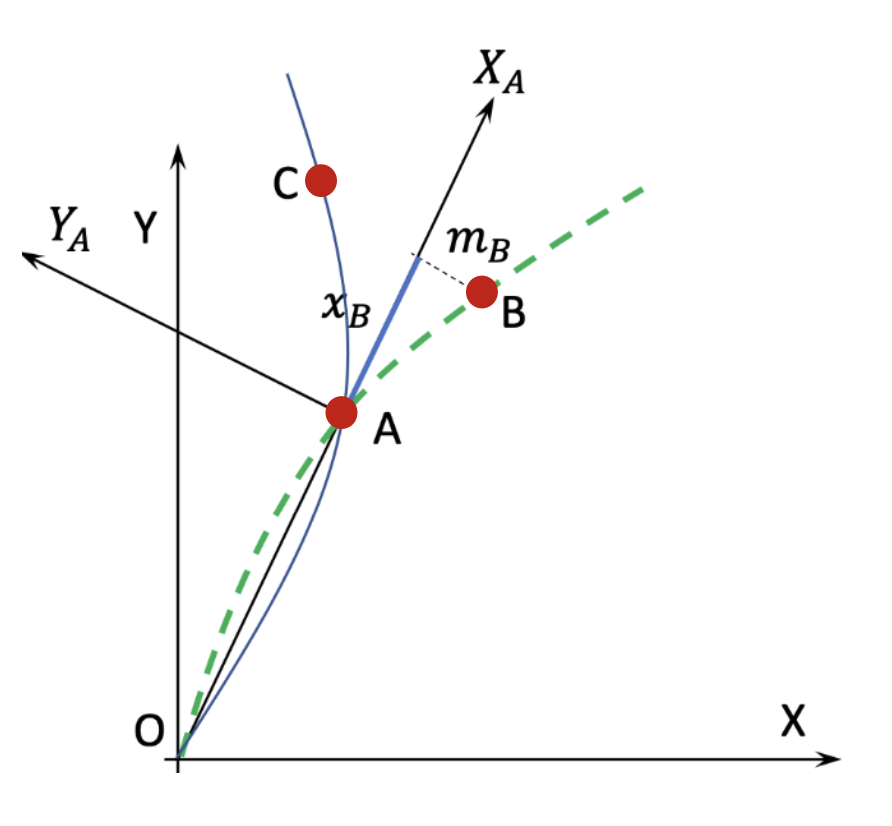
\includegraphics[width=0.42\textwidth]{images/6-trackml/parabolic-state-model-1.png}%
        \label{fig:gnn-parabolic-state-1}%
        }%
    \hfill%
    \subfloat[]{%
        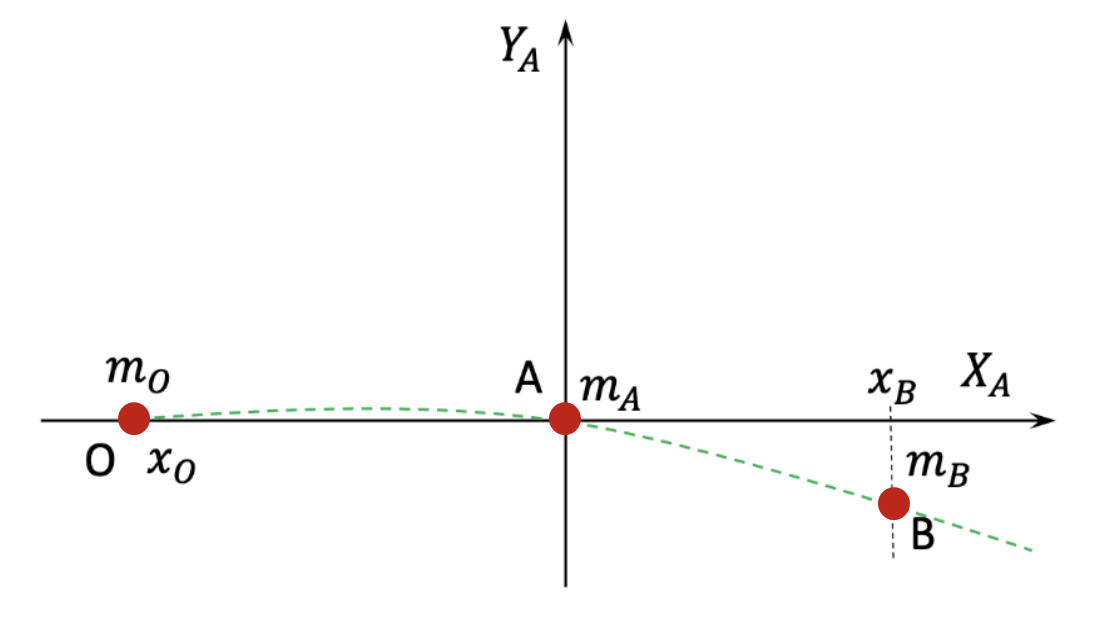
\includegraphics[width=0.56\textwidth]{images/6-trackml/parabolic-state-model-2.png}%
        \label{fig:gnn-parabolic-state-2}%
        }%
    \caption{Parabolic model illustration. a) Construction of example parabolas O - A - B and O - A - C, where O is the global origin and A, B, C are graph nodes. b) Rotation of parabola O - A - B into the local coordinate system of A.}
    \label{fig:gnn-parabolic-model}
\end{figure}


Using the quadratic equation of a parabola, the vector of measurements in the local coordinate system of node A, $ m = [m_O \quad m_A \quad m_B]^{T}$ can be expressed in terms of the unknown parabolic coefficients $p = [a \quad b \quad c]^{T}$ using Eq \eqref{eqn:parabolic-equations}, 

\begin{equation}
    m = H p 
    \label{eqn:parabolic-equations}
\end{equation}

where $m_O$, $m_A$ and $m_B$ are the respective measurements of the global origin O, node A and node B, transformed into the local coordinate system of node A, and $\{a, b, c\}$ are the parabolic coefficients. Measurements $m_O = 0$ and $m_A = 0$, as illustrated in Figure \ref{fig:gnn-parabolic-state-2}. The measurement matrix, $H$, relates the measurement vector, $m$, to the vector of parabolic parameters, $p$, and is given by Eq \eqref{eqn:trackml-matrix-h-xy},

\begin{equation}
    H = \begin{bmatrix} x_O^{2} & x_O & 1 \\ 0 & 0 & 1 \\ x_B^{2} & x_B & 1 \end{bmatrix} 
    \label{eqn:trackml-matrix-h-xy}
\end{equation}

where $x_O$ and $x_B$ are the $x$-coordinates of global origin O and node B in the local coordinate system of node A. The parabolic parameters are derived using Eq \eqref{eqn:derive-p}.

\begin{equation}
    p = H^{-1} m 
    \label{eqn:derive-p}
\end{equation}


% \begin{equation}
% \begin{aligned}
% m_O = ax_{O}^{2} + bx_O + c \\
% m_A = c \\
% m_B = ax_{B}^{2} + bx_B + c
% \end{aligned}
% \label{eqn:parabolic-equations}
% \end{equation}


\subsection{Linear Track Model}
\label{linear-state}

The $r$-$z$ plane is parallel to the direction of the beamline where tracks follow a linear model, as the influence of the solenoidal magnetic field is negligible. The inverse track inclination, $\tau$, between node A and neighbour B, is given by Eq \eqref{eqn:tau-parameter}, where $(z_A, r_A)$ refer to measurements of node A and $(z_B, r_B)$ refer to measurements of neighbour node B.

\begin{equation}
\tau = \frac{z_A - z_B}{r_A - r_B}
\label{eqn:tau-parameter}
\end{equation}

\subsection{Combined Track State Estimate}

Parabolic parameters $\{a, b\}$ derived in Section \ref{parabolic-state}, as well as the inverse track inclination, $\tau$, given in Eq \eqref{eqn:tau-parameter}, provide an indication of track orientation. Hence, the track state estimate, $X_{ij}$, at node $i$ given neighbour $j$ is defined by Eq \eqref{eqn:joint-state-vector}.

\begin{equation}
X_{ij} = \begin{bmatrix} a \\ b \\ \tau \end{bmatrix}
\label{eqn:joint-state-vector}
\end{equation}







\section{Derivation of Edge State Covariance}
\label{chapter-6-covariance-derivation}

To derive the edge state covariance, $C_{ij}$, of $X_{ij}$ given by Eq \eqref{eqn:joint-state-vector}, the covariance of the track state parameters in the $x$-$y$ and $r$-$z$ planes are handled separately. 


\subsection{Covariance of Parabolic Parameters}

The joint measurement covariance matrix, $S_{xy}$, for a parabola constructed in the $x$-$y$ plane using the global origin O and nodes A and B, as illustrated in Figure \ref{fig:gnn-parabolic-state-2}, is stated in Eq. \eqref{eqn:trackml-s-matrix-xy}


\begin{equation}
    S_{xy} = \begin{bmatrix} \sigma_O^{2} & 0 & 0 \\ 0 & \sigma_A^{2} & 0 \\ 0 & 0 & \sigma_B^{2} \end{bmatrix} 
    \label{eqn:trackml-s-matrix-xy}
\end{equation}

where $\sigma_O$, $\sigma_A$ and $\sigma_B$ are the respective errors due to the measurements at the global origin O, node A and node B, using the parabolic model approximation outlined in Section \ref{parabolic-state}. The measurement error in the global origin $\sigma_O$ is initialised to 4.0mm due to the large error in the beamspot, whereas $\sigma_A$ and $\sigma_B$ are initialised to 0.3mm due to the high precision of the Pixel detector. Hence, the covariance of the vector of parabolic parameters, $p$, is given by $C_{xy}$ in Eq \eqref{eqn:c-xy}

\begin{equation}
    C_{xy} = H^{-1}S_{xy}{H^{-1}}^{T}
    \label{eqn:c-xy}
\end{equation}






\subsection{Variance in Inverse Track Inclination}

The joint measurement covariance matrix, $S_{rz}$, for node $i$ and neighbour node $j$ in the $r$-$z$ plane is stated in Eq \eqref{eqn:trackml-s-matrix-rz}, where $\{ \sigma_{zi}, \sigma_{zj} \}$ are the measurement errors along the $z$-axis and $\{ \sigma_{ri}, \sigma_{rj} \}$ are the measurement errors in $r$, for the respective $i$ and $j$ nodes. 

\begin{equation}
    S_{rz} = \begin{bmatrix} \sigma_{zi}^{2} & 0 & 0 & 0 \\ 
                             0 & \sigma_{zj}^{2} & 0 & 0 \\ 
                             0 & 0 & \sigma_{ri}^{2} & 0 \\
                             0 & 0 & 0 & \sigma_{rj}^{2}
                            \end{bmatrix} 
    \label{eqn:trackml-s-matrix-rz}
\end{equation}


The magnitude of the error in the $r$-$z$ plane is dependent on the detector layer where the graph node is situated. For example, for a barrel-located node the error in the $z$-axis will be greater than the error in the $r$-axis due to the orientation of the barrel layer, and vice versa for the endcap. Therefore, for a node located in the Pixel barrel $\sigma_r = 0.4$mm and $\sigma_z = 0.6$mm. For a node located in the Pixel endcap $\sigma_r = 0.6$mm and $\sigma_z = 0.4$mm

The error in the track inclination $\tau$ is computed using the standard error propagation and linear algebra approach. The transition Jacobian, $G$, relates the measurements in the $r$-$z$ plane to the inverse track inclination $\tau$ and is given by Eq \eqref{trackml-g-rz}.

% this applies to either node i or node j
% sigma0r = 0.4 --> error in r for barrel located node
% sigma0r = 0.6 --> error in r for endcap located node

% sigma0z = 0.6 --> error in z for barrel located node
% sigma0z = 0.4 --> error in z for endcap located node


\begin{equation}
    G = \begin{bmatrix} 
            (r_i - r_j)^{-1} &
            -(r_i - r_j)^{-1} & 
            \frac{-(z_i - z_j)}{(r_i - r_j)^2} & 
            \frac{z_i - z_j}{(r_i - r_j)^2}
            \end{bmatrix} 
    \label{trackml-g-rz}
\end{equation}

The corresponding error in track inclination $\tau$ is given by Eq \eqref{eqn:error-in-tau}

\begin{equation}
    \sigma_{\tau} = G S_{rz} G^{T}
    \label{eqn:error-in-tau}
\end{equation}






\subsection{Moli\`ere Theory of Multiple Scattering}

A charged particle traversing a medium is deflected by many small-angle scatters. Most of this deflection is due to Coulomb scattering from nuclei. However, for hadronic projectiles the strong interactions also contribute to multiple scattering. Therefore, the error in track direction will have a contribution from the observed error due to multiple scattering, $\sigma_{ms}$. According to the theory of Moli\`ere, the scattering distribution is roughly Gaussian for small deflection angles. The contribution due to Moli\`ere multiple scattering is given by the simplified Highland formula \cite{moliere-theory-formula, Lynch:1990sq} stated in Eq \eqref{eqn:simplified-moliere-equation}.

%The Moli\`ere multiple scattering is inversely proportional to particle full momentum and proportional to the square root of material thickness.

% \begin{equation}
%     \sigma_{ms}^{2} = \frac{13.6 \text{MeV}}{\beta c p} z \sqrt{\frac{x}{X_0}} \left[ 1 + 0.038ln \left( \frac{x}{X_0} \right) \right] 
%     \label{eqn:moliere-equation}
% \end{equation}

\begin{equation}
    \sigma_{ms}^{2} = \frac{13.6 \text{MeV}}{\beta c p} z \sqrt{\frac{x}{X_0}}
    \label{eqn:simplified-moliere-equation}
\end{equation}

where $p$, $\beta c$, and $z$ are the full momentum, velocity, and charge number of the incident particle, and $x/X_0$ is the thickness of the scattering medium, measured in radiation lengths. For a realistic particle, $\beta c \approx 1$ and the charge, $z$, is assumed to be 1. 




\subsubsection{Derivation of Full Momentum}

The full particle momentum, $p$, is given by Eq \eqref{eqn:full-momentum}

\begin{equation}
    p = p_\text{T} / \sin(\theta)
    \label{eqn:full-momentum}
\end{equation}

where $p_\text{T}$ is the transverse momentum of the particle and $\theta$ is the angle of inclination of the particle trajectory to the $z$-axis. The transverse momentum, $p_\text{T}$, for a charged particle in the presence of a magnetic field is given by Eq \eqref{eqn:transverse-momentum}

\begin{equation}
    p_\text{T} [\text{MeV}] = 0.3 B [\text{T}] \times q [\text{e}] \times r [\text{mm}]
    \label{eqn:transverse-momentum}
\end{equation}

where $p_\text{T}$ is measured in GeV/c. The magnetic field strength of the TrackML model is given by $B$, the charge of the particle is given by $q$ and is set to 1, and $r$ is the radius which is inversely proportional to the track curvature $\kappa$, given by Eq \eqref{eqn:kappa}, 

\begin{equation}
\kappa = \frac{2a}{(1 + (2ax + b)^2)^{\frac{3}{2}}}
\label{eqn:kappa}
\end{equation}

where $\kappa$ is a function of parabolic parameters $a$ and $b$, and $x$ is the $x$-coordinate of the point at which the curvature is calculated. Therefore, the full momentum $p$ is hence given by Eq \eqref{eqn:full-momentum-derived} using the knowledge that $\kappa = 1/r$.

\begin{equation}
p = 0.3 B / \kappa \sin(\theta)
\label{eqn:full-momentum-derived}
\end{equation}

where $B$ = 2T, modelling the magnetic field strength of the TrackML detector.

\subsubsection{Orientation of Detector Layers}

If a particle crosses one of the TrackML detector layers at incident angle $\theta$, then the radiation length, $x/X_0$, is given by Eq \eqref{eqn:radiation-length}

\begin{equation}
x/X_0 = 0.02 f(\theta)
\label{eqn:radiation-length}
\end{equation}

where 0.02 is the integrated $x/X_0$ for a typical silicon detector layer which is considered as a single thin scatter. The function $f(\theta)$ is determined by the orientation of the detector layer, on which the node-pair is located. For example, for a scattered node in the Pixel barrel layer $f(\theta) = 1 / \sin(\theta)$, and for a scattered node in the Pixel endcap layer $f(\theta) = 1 / \cos(\theta)$.




\subsubsection{Variance of Multiple Scattering}

The final form of the observed contribution of error due to multiple scattering is $\sigma_{ms}$, where the variance, $\sigma_{ms}^2$, is given by Eq \eqref{eqn:computed-multiple-scattering}.

\begin{equation}
    \sigma_{ms}^{2} = \frac{13.6 \text{MeV}}{B} \cdot 0.02 f(\theta) \cdot \kappa \sin(\theta)
    \label{eqn:computed-multiple-scattering}
\end{equation}



\subsection{Combined Edge State Covariance}

The edge state covariance matrix of the combined track state estimate $X_{ij}$, is given by $C_{ij}$ in Eq \eqref{eqn:combined-edge-state-covariance}.

\begin{equation}
    C_{ij} = \begin{bmatrix} 
            C_{xy}^{00} & C_{xy}^{01} & 0 \\ 
            C_{xy}^{10} & C_{xy}^{11} + \sigma_{ms}^2 & 0 \\ 
            0 & 0 & \sigma_{\tau}^{2} + \sigma_{ms}^2 \\
            \end{bmatrix} 
    \label{eqn:combined-edge-state-covariance}
\end{equation}

where $C_{xy}^{00}$, $C_{xy}^{01}$, $C_{xy}^{10}$ and $C_{xy}^{11}$ are the corresponding matrix components of the covariance of the vector of parabolic parameters $p$, $C_{xy}$, in the $x$-$y$ plane, stated in Eq \eqref{eqn:c-xy}, and $\sigma_{\tau}^2$ is the variance of the inverse track inclination $\tau$, stated in Eq \eqref{eqn:error-in-tau}. The combined edge state covariance, $C_{ij}$, is therefore represented as a 2 $\times$ 2 block matrix of the $[cov(a, b)]$ extracted from $C_{xy}$, and the variance in $\tau$.

The non-diagonal elements of $C_{ij}$ in the third dimension are zero as there is no correlation in measurements between the $x$-$y$ and $r$-$z$ plane for the Pixel detector.

Components of $X_{ij}$, that represent the error in track direction must have a contribution from the observed error due to multiple scattering, $\sigma_{ms}$. Therefore, the variance due to multiple scattering, $\sigma_{ms}^2$ must be added to the variance of parameters $b$ and $\tau$, represented by matrix components $C_{ij}^{11}$ and $C_{ij}^{22}$.




\section{Learning the Optimal KL Threshold}
\label{chapter-6-kl-threshold}

During stage 1 of the GNN algorithm, GMR via k-means clustering is used to reduce the Gaussian mixture of states, $g_i(X)$, at each node $i$. In order to establish if track state estimates, $X_{ij}$, can be grouped into a cluster, the KL divergence, $d_{KL}$, is used as a threshold distance as it is a measure of the statistical distance between two Gaussian probability distributions \cite{KL, FRUHWIRTH19971}.

To determine the optimal pairwise $d_{KL}$ between $X_{ij}$ for a given node, a SVM classifier was trained. Pairwise $d_{KL}$ and the empirical variance of edge orientation, $\sigma_{e}^{2}$, for a given node are used as input features. Figure \ref{fig:KL-distance-truth} shows the ground truth data of these input features from $10,000$ MC simulated particle collision events, each event with ten truth tracks. Loosely compatible edge connections were formed using a hit-pair predictor based on track inclination angle of neighbouring hits, similar to the graph network constructed in \ref{fig:heat-map}. The feature vector was comprised of $\sigma_{e}$ for a given node and pairwise $d_{KL}$ between its track states. The truth particle was extracted for each pairwise connection. For a given pair of edge connections with a common node, truth 1 corresponds to all nodes originate from the same truth particle, and truth 0 corresponds to otherwise. 

%The truth data is presented is Figure \ref{fig:KL-distance-truth}.

A SVM was trained to discriminate between the two classes \cite{scikit-learn}, using a polynomial degree three kernel. SVM predictions are shown in Figure \ref{fig:KL-distance-predictions} and were adjusted such that the TPR was tuned to 95\% in order to maintain a high purity. The SVM decision boundary was converted into a fast LUT using a similar methodology outlined in Section \ref{LUT-generation} and was directly used within the k-means clustering of the GMR stage. If $d_{KL}$ is less than the predicted threshold for a node with a given $\sigma_e$, then the pairwise states are clustered together and merged into a single state $X^M$.

% The predictions and corresponding decision boundary is shown in Figure \ref{fig:KL-distance-predictions}.

Other classification algorithms were explored, however the SVM was the most appropriate to determine a decision boundary to best separate the classes.

\begin{figure}[htbp!] 
    \centering
    \subfloat[Ground Truth Data from MC Simulation]{%
        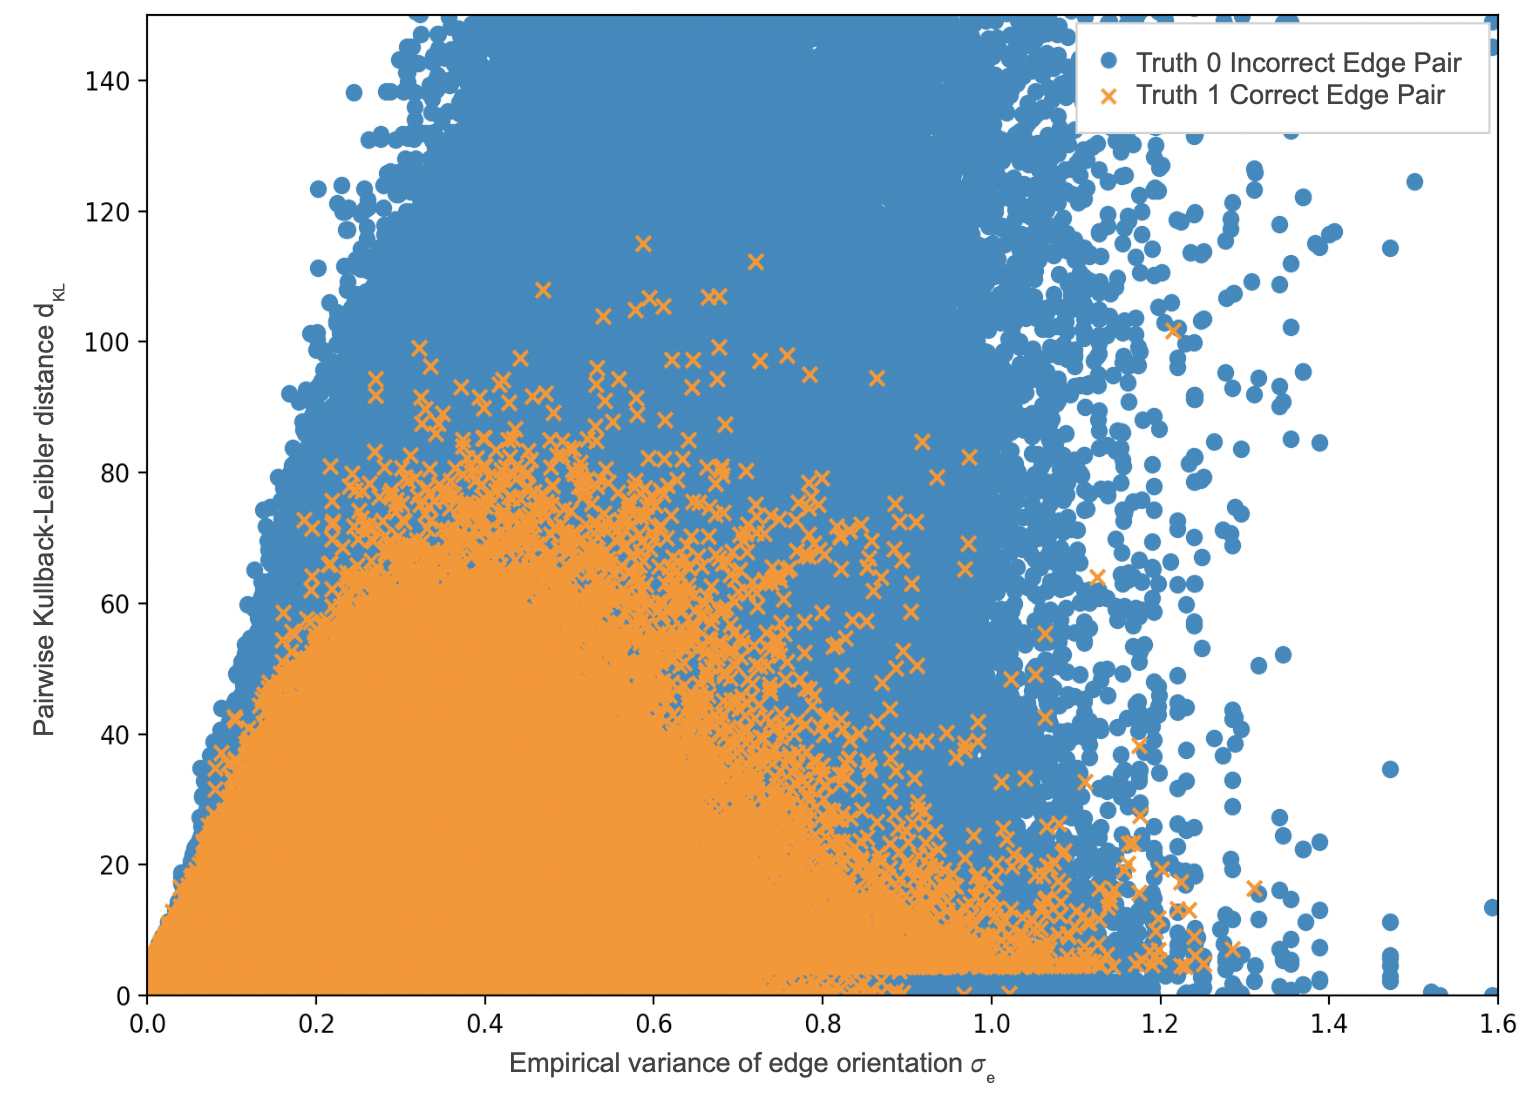
\includegraphics[width=0.82\linewidth]{images/6-trackml/kl-truth.png}%
        \label{fig:KL-distance-truth}%
        }%
    \hfill%
    \subfloat[SVM Predictions and Decision Boundary (dotted line)]{%
        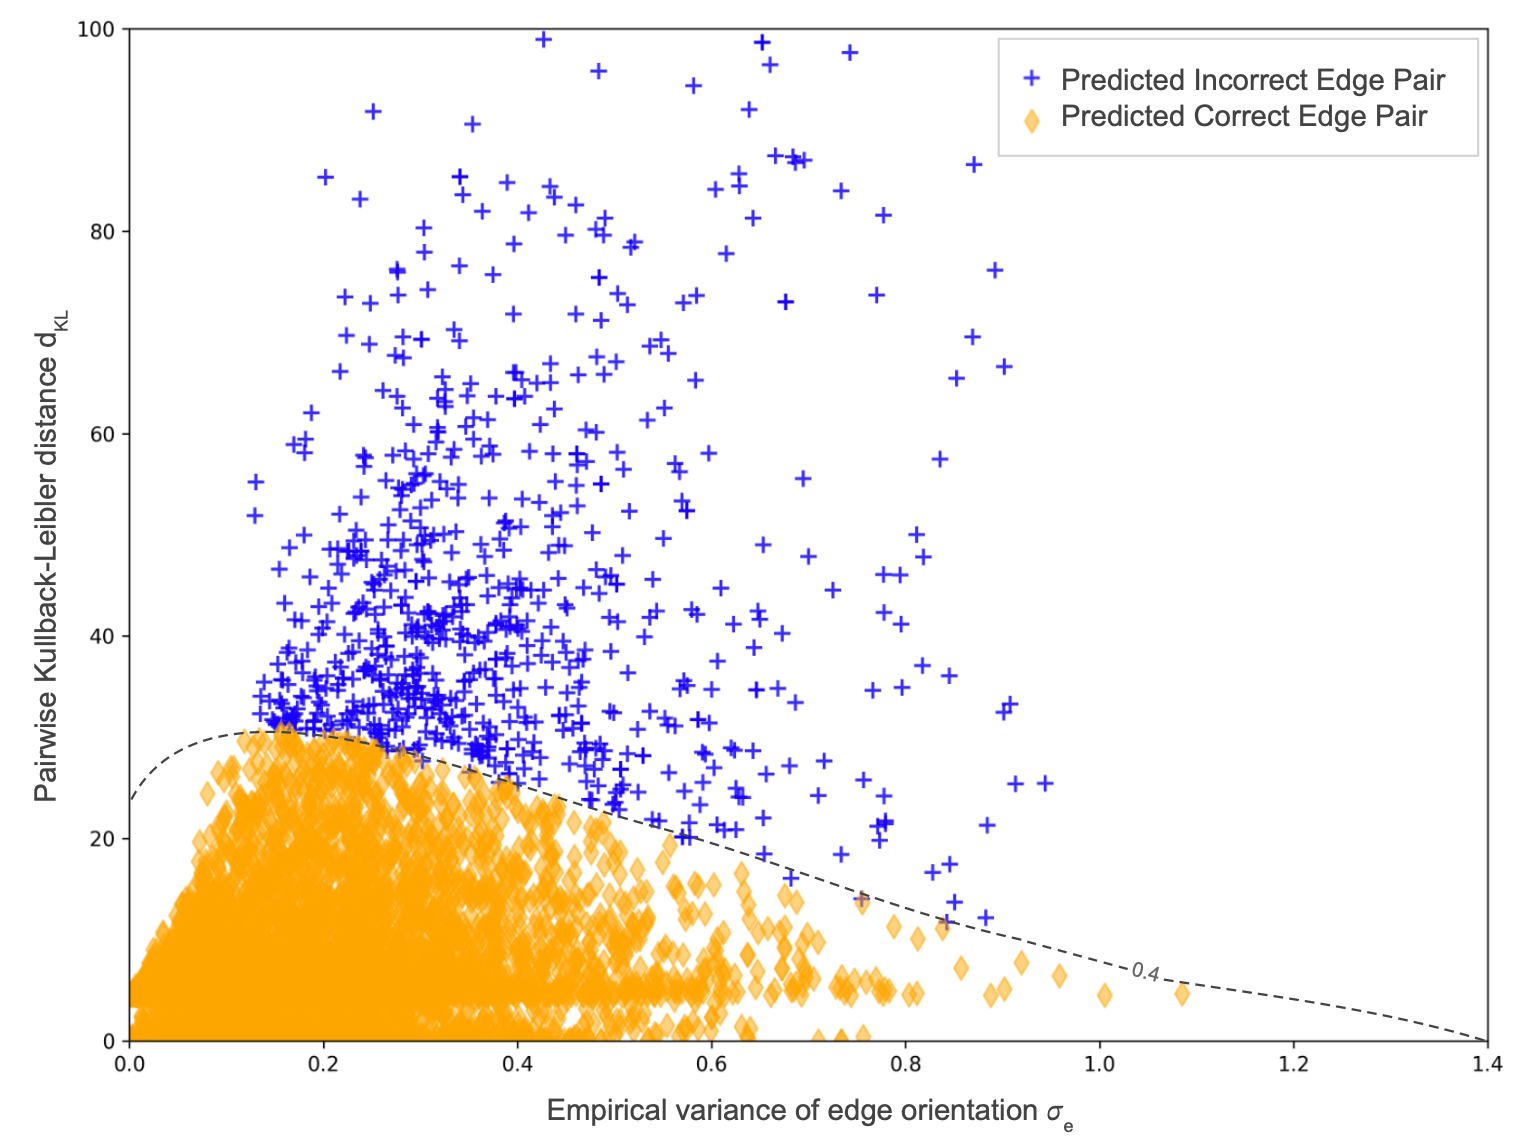
\includegraphics[width=0.82\linewidth]{images/6-trackml/kl-predictions.png}%
        \label{fig:KL-distance-predictions}%
        }%
    \caption{SVM classifier training and predictions used to determine the optimal Kullback-Leibler threshold distance, $d_{KL}$, between pairwise track states $X_{ij}$, for a given node with a variance of edge orientation $\sigma_e$. The dotted line in b) represents the threshold value of 0.40 when adjusting SVM predictions in order to yield a TPR of 95\%. For a given pair of edge connections with a common node, truth 1 corresponds to all nodes originate from the same truth particle, and truth 0 corresponds to otherwise.}
    \label{fig:KL-distance}
\end{figure}













\section{Extrapolation and Track Extraction}
\label{chapter-6-extrapolation-track-extraction}

\subsection{Overview of KF Implementation}
\label{chapter-6-overview-of-kf}

Extrapolation and track extraction are handled independently for the $x$-$y$ and $r$-$z$ planes, with each stage using a separate KF. The filter parameters are summarized in Table \ref{tab:kf-instance-variables} and the derivations are described in Sections \ref{chapter-6-start-of-derivation} - \ref{chapter-6-end-of-derivation}.



\begin{table}[!htbp]
\caption{Summary of parameters used in the implementation of KFs for state extrapolation and track extraction, in the $x$-$y$ and $r$-$z$ planes.}
\begin{center}
\begin{tabular}{lccc}
\toprule
& \multicolumn{3}{c}{Parameters for $x$-$y$ Plane} \\
Instance Variable Description & Symbol  & Extrapolation  & Track Extraction  \\
\hline
\rule{0pt}{3ex}%

Filter State Estimate
& $\hat{x}_{xy}$
& $\tilde{X}_{xy}$
& $\begin{bmatrix} m'_{(n-1)} & \tau'_{xy} & w_{ou} \end{bmatrix}^{T}$
\\
\rule{0pt}{4ex}%

Filter State Covariance
& $\hat{P}_{xy}$ 
& $\tilde{C}_{xy}$ 
& $\begin{bmatrix} \sigma_{xy}^2 & 0 & 0 
                   \\ 0 & \sigma_{\tau_{xy}}^2 & 0 
                    \\ 0 & 0 & \sigma_{w_{ou}}^2 \end{bmatrix}$
\\
\rule{0pt}{4ex}%

State Transition Jacobian
& $\hat{F}_{xy}$ 
& $\begin{bmatrix} 
        \frac{\partial a'}{\partial a} & \frac{\partial a'}{\partial b} & \frac{\partial a'}{\partial c} \\ 
        
        \frac{\partial b'}{\partial a} & \frac{\partial b'}{\partial b} & \frac{\partial b'}{\partial c} \\
        
        \frac{\partial c'}{\partial a} & \frac{\partial c'}{\partial b} & \frac{\partial c'}{\partial c} \\
        \end{bmatrix}$
& $\begin{bmatrix} 1 & dx' & g_1 \\ 0 & 1 & f_1 \\ 0 & 0 & e_1 \end{bmatrix} $
\\
\rule{0pt}{3ex}%


Measurement Function
& $\hat{H}_{xy}$ 
& \multicolumn{2}{c}{$[0 \quad 0 \quad 1]$}
\\
\rule{0pt}{3ex}%

Measurement Uncertainty
& $\hat{R}_{xy}$ 
& \multicolumn{2}{c}{$\sigma_{xy}^{2}$}
\\
\rule{0pt}{6ex}%

Process Noise
& $\hat{Q}_{xy}$ 
&  $\begin{bmatrix} 0 & 0 & 0 \\ 
                    0 & \sigma_{ms}^2 & 0 \\
                    0 & 0 & 0 \end{bmatrix}$ 
& $\begin{bmatrix} Q_{00} & Q_{01} & Q_{02} \\  Q_{01} & Q_{11} & Q_{12} \\ Q_{02} & Q_{12} & Q_{22} \end{bmatrix} $ 
\\


\bottomrule
\rule{0pt}{3ex}%
& \multicolumn{3}{c}{Parameters for $r$-$z$ Plane} \\
Instance Variable Description & Symbol  & Extrapolation  & Track Extraction  \\
\hline
\rule{0pt}{3ex}%


Filter State Estimate
& $\hat{x}_{rz}$
& $\begin{bmatrix} m_i & \tau_{ij} \end{bmatrix}^{T}$
& $\begin{bmatrix} z_{(n-1)} & \tau_{(n-1)} \end{bmatrix}^{T}$
\\
\rule{0pt}{4ex}%

Filter State Covariance
& $\hat{P}_{rz}$ 
& \multicolumn{2}{c}{$\begin{bmatrix} \sigma_{rz}^2 & 0 \\ 0 & \sigma_{\tau}^2 + \sigma_{ms}^2 \end{bmatrix}$}
\\
\rule{0pt}{4ex}%

State Transition Jacobian
& $\hat{F}_{rz}$ 
& \multicolumn{2}{c}{$\begin{bmatrix} 1 & dr \\ 0 & 1 \end{bmatrix}$}
\\
\rule{0pt}{3ex}%

Measurement Function
& $\hat{H}_{rz}$ 
& \multicolumn{2}{c}{$[1 \quad 0]$}
\\
\rule{0pt}{3ex}%

Measurement Uncertainty
& $\hat{R}_{rz}$ 
& \multicolumn{2}{c}{$\sigma_{rz}^2$}
\\
\rule{0pt}{3ex}%

Process Noise
& $\hat{Q}_{rz}$ 
& \multicolumn{2}{c}{$\sigma_{ms}^2$}
\\  
              

\bottomrule

\end{tabular}
\end{center}
\label{tab:kf-instance-variables}
\end{table}










\subsection{Parabolic Extrapolation Model for x-y Plane}
\label{chapter-6-start-of-derivation}

A parabolic model for state extrapolation is used for the transverse $x$-$y$ plane. We begin with a parabola connecting the global origin O to node A, in the local coordinate system of node A given by axis $(X_A, Y_A)$, illustrated by Figure \ref{fig:trackml-parabolic-extrapolation-model-xy}.

\begin{figure}[htbp]
    \centering
    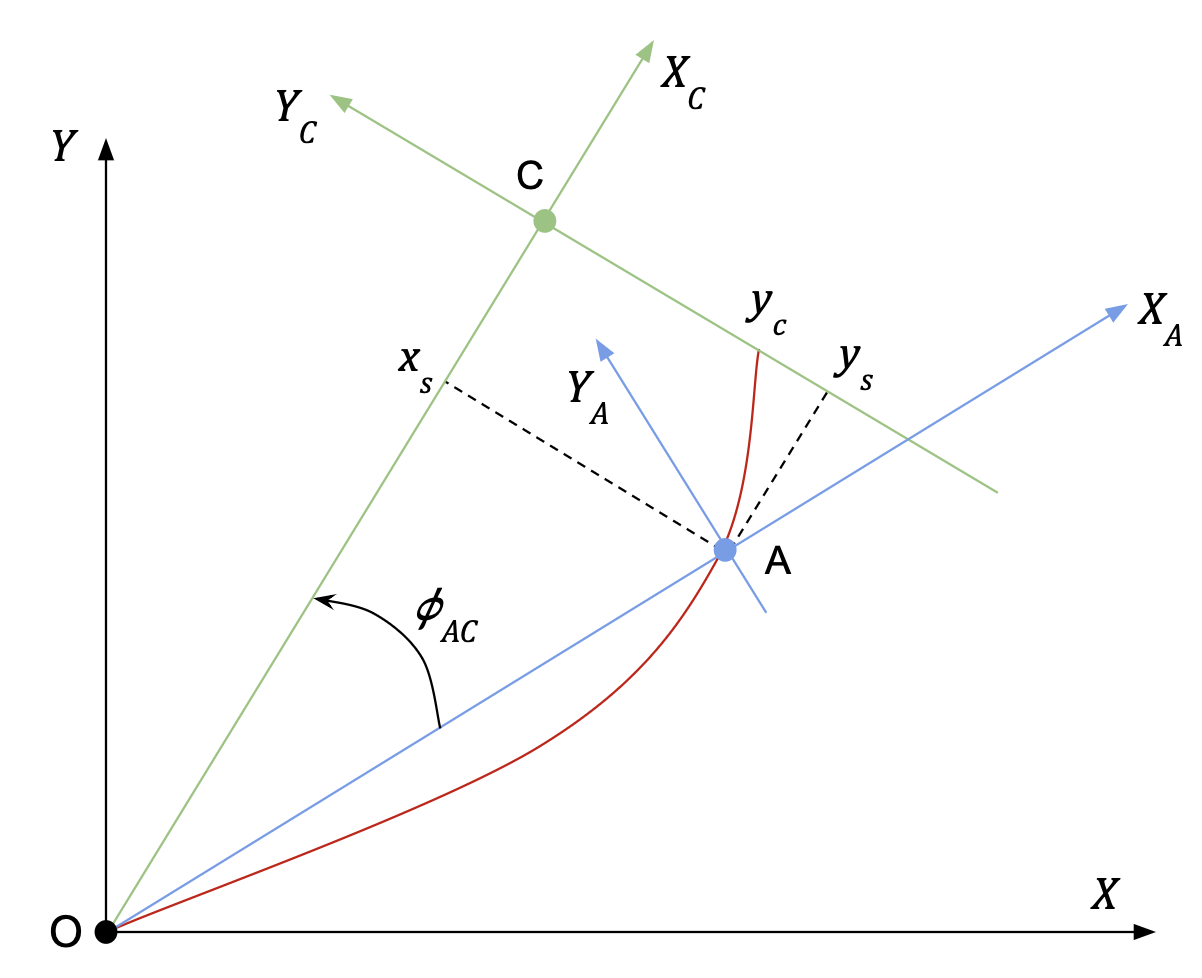
\includegraphics[width=0.7\textwidth]{images/6-trackml/extrapolation-model-xy-trackml-2.png}
    \caption{Illustration of the parabolic extrapolation model used from starting node A and to target node C. The angle of rotation between node A and node C is given by $\phi_{AC}$. The parabola (red) connects the global origin O to node A.}
    \label{fig:trackml-parabolic-extrapolation-model-xy}%
\end{figure}

The parabola has known parameters, $\{a, b, c\}$, derived during previous stages of the algorithm and can be represented in parametric form local to node A, given by Eqs \eqref{eqn:parabolic-equations-parametric}.

\begin{equation}
\begin{aligned}
y_A(u) = au^{2} + bu + c \\
x_A(u) = u
\end{aligned}
\label{eqn:parabolic-equations-parametric}
\end{equation}

The target node for state extrapolation is node C, which has its own local coordinate system given by axis $(X_C, Y_C)$, and is also described by a parabola. In parametric form, the parabola at node C is given by Eqs \eqref{eqn:parabolic-equations-parametric-nodeC}.

\begin{equation}
\begin{aligned}
y_C(v) = a'v^{2} + b'v + c' \\
x_C(v) = v
\end{aligned}
\label{eqn:parabolic-equations-parametric-nodeC}
\end{equation}

where $\{a', b', c' \}$ are the parabolic parameters in the local coordinate system of node C. The transformation from the local coordinate system of node A to the coordinate system local to node C is given by Eqs \eqref{eqn:rotation-parabolic-linear-algebra}. First a rotation is applied, through angle $\phi_{AC}$ describing the global angle between node A and node C, followed by a translation adding the corresponding shifts $x_s$ and $y_s$.

\begin{equation}
\begin{aligned}
x_C = x_s + u\cos(\phi_{AC}) + (au^2 + bu + c)\sin(\phi_{AC}) \\
y_C = y_s - u\sin(\phi_{AC}) + (au^2 + bu + c)\cos(\phi_{AC})
\end{aligned}
\label{eqn:rotation-parabolic-linear-algebra}
\end{equation}

% the extrapolation ends when this condition is met (target condition

The extrapolation ends when $x_{C}(u) = 0$, as can be seen in Figure \ref{fig:trackml-parabolic-extrapolation-model-xy} when the parabola crosses the $Y_C$ axis. This condition forms a quadratic equation in $u$, where the solution $u^{*} = u(a, b, c)$. Using parametric derivatives, the parabolic parameters $\{a’, b’, c’ \}$ in the coordinate system of the target node, C, can be derived in terms of parabolic parameters $\{a, b, c \}$ in the coordinate system of the starting node, A at the boundary condition $x_{C}(u) = 0$. The Jacobian is then calculated by differentiation of the formulas for $\{a’, b’, c’ \}$ with respect to initial parameters $\{a, b, c \}$, given by Eq \eqref{eqn:transition-jacobian-F-kf-extrapolation-xy}.  

% quadratic equation in s, where the solution s* is a function of the parabolic parameters local to node A. We then have a function s* as a function of a, b, c


\begin{equation}
\hat{F}_{xy} = \begin{bmatrix} 
        \frac{\partial a'}{\partial a} & \frac{\partial a'}{\partial b} & \frac{\partial a'}{\partial c} \\ 
        
        \frac{\partial b'}{\partial a} & \frac{\partial b'}{\partial b} & \frac{\partial b'}{\partial c} \\
        
        \frac{\partial c'}{\partial a} & \frac{\partial c'}{\partial b} & \frac{\partial c'}{\partial c} \\
        \end{bmatrix} 
\label{eqn:transition-jacobian-F-kf-extrapolation-xy}
\end{equation}


The extrapolated track state, $\tilde{X}_{xy}$, and extrapolated covariance, $\tilde{C}_{xy}$, are calculated using $F_{xy}$ and Eqs \eqref{eqn:extrapolation}, where the process noise, $Q_{xy}$, is given by Eq \eqref{eqn:process-noise-Q-extrapolation-xy}.

\begin{equation}
\hat{Q}_{xy} = \begin{bmatrix} 
                0 & 0 & 0 \\ 
                0 & \sigma_{ms}^2 & 0 \\
                0 & 0 & 0 \end{bmatrix} 
\label{eqn:process-noise-Q-extrapolation-xy}
\end{equation}

The residual, $r$, between the projection of the extrapolated state and the measurement at node C is calculated using Eq \eqref{eqn:residual-trackml-xy}

\begin{equation}
r = m_C - \hat{H}_{xy} \tilde{X}
\label{eqn:residual-trackml-xy}
\end{equation}

where $\hat{H}_{xy} = [0, 0, 1]$ and $m_C$ is the $y$-coordinate of node C in its local coordinate system, hence $m_C = 0$. The covariance of the residual, $V$ , is given by Eq \eqref{eqn:covariance-of-residual-trackml-xy}

\begin{equation}
{V} = \hat{H}_{xy} \widetilde{C} \hat{H}^{T}_{xy} + \sigma_{xy}^{2}
\label{eqn:covariance-of-residual-trackml-xy}
\end{equation}

where $\sigma_{xy} = 300\mu$m. The corresponding Mahalanobis distance, $\Delta \chi^{2}$, is given by Eq \eqref{eqn:mahalanobis-distance-trackml-xy}, and the distributions can be seen in Figure \ref{fig:mahalanobis-threshold-trackml-xy}.

\begin{equation}
\Delta \chi^{2} = r^{T} {V}^{-1} r
\label{eqn:mahalanobis-distance-trackml-xy}
\end{equation}


\begin{figure}[htbp]
    \centering
    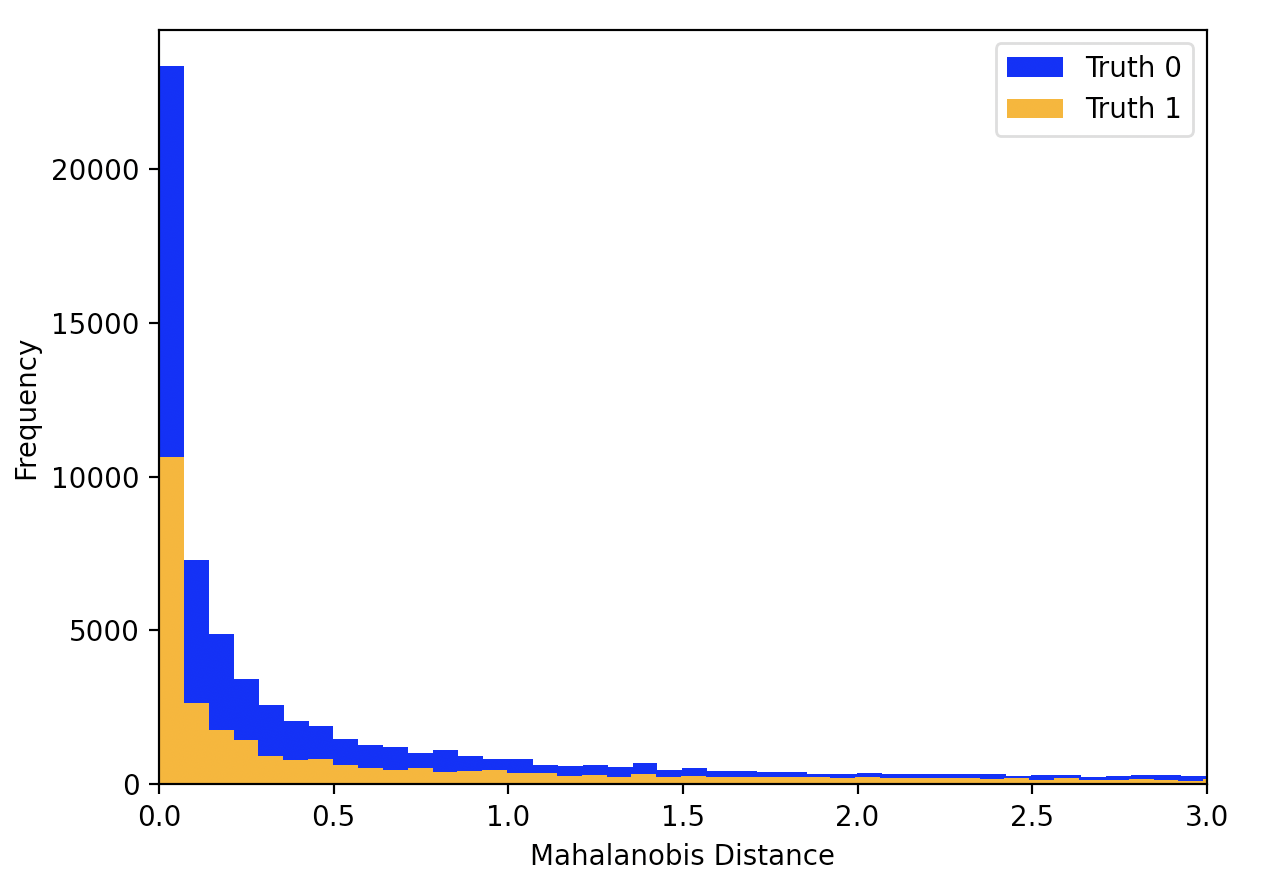
\includegraphics[width=0.85\textwidth]{images/6-trackml/mahalanobis-threshold-trackml-xy.png}
    \caption{Mahalanobis distance, $\Delta \chi^{2}$, computed between the projected state and the measurement at each node for the GNN algorithm applied to the TrackML model during state extrapolation in the $x$-$y$ plane. Truth 1 shows the distribution where the truth particle originating from the extrapolated state and the truth particle originating from the measurement are the same, and truth 0 otherwise.}
    \label{fig:mahalanobis-threshold-trackml-xy}%
\end{figure}


A threshold cut of 1 is used such that a high purity of truth 1 edge connections are maintained. If $\Delta \chi^{2} < 1$, then $\tilde{X}$ is fully extrapolated to its neighbour node using the KF update.



%\subsubsection{KF Setup for State Extrapolation}

The KF for state extrapolation is initialised with filter state estimate set to the extrapolated track vector, $\hat{x}_{xy} = \tilde{X}_{xy}$, and similarly the filter covariance, $\hat{P}_{xy} = \tilde{C}_{xy}$. The KF is also initialised with the Jacobian in Eq \eqref{eqn:transition-jacobian-F-kf-extrapolation-xy} and process noise in Eq \eqref{eqn:process-noise-Q-extrapolation-xy}. The measurement error, $\hat{R}$, is attributed to the error due to the measurement of the $x$-$y$ plane and is set to $\sigma_{xy} = 300\mu$m.










\subsection{KF Setup for Track Extraction in x-y Plane}
%The KF track fit is applied simultaneously in both the $x$-$y$ and $r$-$z$ planes, in order to assess the quality of the fit using both models. In comparison to the KF used for state extrapolation (Section \ref{kf-for-extrp-chapter-6}), the KF for track fitting considers the entire chain of track segments making up a track candidate. Therefore, there will be a non-zero process noise, $Q$, present in both $x$-$y$ and $r$-$z$ planes.

The KF works in a rotated coordinate system, whereby the first track segment in the chain of segments representing a track candidate is rotated to be parallel to the global $x$-axis. This rotated coordinate system is denoted by $(x', y')$, not to be confused with the global coordinate system $(x, y)$. The new $x$-axis, $x'$, is parallel to the first track segment and the new $y$-axis, $y'$, describes the track deviation from the straight line.

The KF in the $(x', y')$ plane must take into account the influence of the magnetic field. As the track bends in a particular direction, dependent on the charge of the particle, the magnetic field creates a systematic effect on the track direction and hence a near-constant drift in the azimuthal angle from the $x$-axis, $\phi$. Statistically, such a situation can be described as a correlated noise which affects the track direction and can be modelled by the Ornstein-Uhlenbeck (OU) process \cite{OU}. Using the OU process, the track direction evolves stochastically according to a deterministic drift parameter, $\alpha$, and stochastic noise, $\sigma_{ou}$. The result is one which can be substituted into the KF as a sophisticated process noise, making the KF track fit three-dimensional.

For a set of $n$ nodes representing a track candidate, the sequential set of measurements are $\{m'_{(n-1)}, ..., m'_1, m'_0, \}$, where $m'_{(n-1)}$ is the measurement of the node with the largest radius, as the track extraction works from the outermost node. The KF is initialised with the following three-dimensional filter state estimate, $\hat{x}_{xy}$, given by Eq \eqref{eqn:kf-track-fit-initialised-state-xy}.


\begin{equation}
\hat{x}_{xy} = \begin{bmatrix} m'_{(n-1)} \\ \tau'_{xy} \\ w_{ou} \end{bmatrix} 
\label{eqn:kf-track-fit-initialised-state-xy}
\end{equation}

where the measurement $m'_{(n-1)}$ is known, $\tau'_{xy}$ is the track inclination in the $(x', y')$ coordinate system initialized to zero and $w_{ou}$ is the integrated OU parameter, also initialized to zero. The filter covariance matrix, $\hat{P}_{xy}$, is initialized using Eq \eqref{eqn:kf-track-fit-initialised-cov-xy}

\begin{equation}
\hat{P}_{xy} = \begin{bmatrix} \sigma_{xy}^2 & 0 & 0 
                            \\ 0 & \sigma_{\tau_{xy}}^2 & 0 
                            \\ 0 & 0 & \sigma_{w_{ou}}^2 \end{bmatrix} 
\label{eqn:kf-track-fit-initialised-cov-xy}
\end{equation}

where $\sigma_{\tau_{xy}}$ is the error in the track inclination, $\tau_{xy}$, and is initialized to 1, and $\sigma_{w_{ou}}$ is the error in the integrated OU parameter, $w_{ou}$, initialized to 1. The state transition Jacobian $\hat{F}_{xy}$ is derived by integration of the OU motion model \cite{OU} and is given by \eqref{eqn:state-transition-jacobian-ou},

\begin{equation}
\hat{F}_{xy} = \begin{bmatrix} 1 & dx' & g_1 \\ 0 & 1 & f_1 \\ 0 & 0 & e_1 \end{bmatrix} 
\label{eqn:state-transition-jacobian-ou}
\end{equation}

where $dx'$ is the difference in $x'$ position of sequential nodes $i$ and $j$ processed in the the KF, $dx' = x'_i - x'_j$, and $e_1$, $f_1$ and $g_1$ are given by the following equations. 

\begin{equation}
e_1 = e^{- \alpha \lvert dx' \rvert}
\label{eqn:e1}
\end{equation}

\begin{equation}
f_1 = \frac{1 - e_1}{\alpha}
\label{eqn:f1}
\end{equation}

\begin{equation}
g_1 = \frac{\lvert dx' \rvert - f_1}{\alpha}
\label{eqn:g1}
\end{equation}

The inverse of the deterministic drift parameter, $\alpha^{-1}$, is proportional to the rate of change of the track azimuthal angle, $\phi$, and is initialised to 0.1. If $\alpha \rightarrow \infty$ the track model becomes a straight line, however if $\alpha \rightarrow 0$, the model becomes a parabola. The process noise, $\hat{Q}_{xy}$, is derived using the OU motion model \cite{OU} and is given by Eq \eqref{eqn:process-noise-q}, 
 
\begin{equation}
\hat{Q}_{xy} = \begin{bmatrix} Q_{00} & Q_{01} & Q_{02} \\  Q_{01} & Q_{11} & Q_{12} \\ Q_{02} & Q_{12} & Q_{22} \end{bmatrix} 
\label{eqn:process-noise-q}
\end{equation}

where the corresponding matrix elements are given by the following equations.

\begin{equation}
Q_{00} = (dx')^{2} (\sigma_{ms}^{2} + \frac{(dx')^{2} \sigma_{ou}^{2}}{4})
\label{eqn:q00}
\end{equation}


\begin{equation}
Q_{01} = dx'( \sigma_{ms}^2 + Q_{02} )
\label{eqn:q01}
\end{equation}

\begin{equation}
Q_{02} = \frac{1}{2} (dx')^2 \sigma_{ou}^{2}
\label{eqn:q02}
\end{equation}

\begin{equation}
Q_{12} = dx' \sigma_{ou}^{2}
\label{eqn:q12}
\end{equation}

\begin{equation}
Q_{11} = \sigma_{ms}^2 + (dx')^{2} \sigma_{ou}^{2}
\label{eqn:q22}
\end{equation}

\begin{equation}
Q_{22} = \sigma_{ou}^2
\label{eqn:q22}
\end{equation}

The process noise, $\hat{Q}_{xy}$, is implemented with the addition of a non-zero stochastic noise, $\sigma_{ou}$, as well as the non-zero error due to the multiple scattering, $\sigma_{ms}$. This represents the correlated noise and models the track curvature caused by the presence of the magnetic field. The stochastic noise, $\sigma_{ou}$, is initialised to $10^{-5}$ and $\sigma_{ms}$ is derived using Eq \eqref{eqn:computed-multiple-scattering}. The measurement error in the KF, $\hat{R}_{xy}$ is attributed to the error due to the measurement of the $x$-$y$ plane and is initialised to $\sigma_{xy} = 300\mu$m.















\subsection{Linear Extrapolation Model for r-z Plane}
\label{chapter-6-r-z-plane-impl}


Similar to Section \ref{gnn-application-toy-model}, a linear model is used for track state extrapolation in the $r$-$z$ plane. Each connection is modelled as a straight line, where the state to extrapolate, $x_{rz}$, from node $i$ to neighbour node $j$ comprises of the $z$-position at node $i$, $m_i$, and the track inclination to node $j$, $\tau_{ij}$, extracted from the combined track state estimate, $X_{ij}$, described at node $i$. The state to extrapolate, $x_{rz}$, is given by Eq \eqref{eqn:track-state-estimate-rz}.

\begin{equation}
x_{rz} = \begin{bmatrix} m_i \\ \tau_{ij} \end{bmatrix}
\label{eqn:track-state-estimate-rz}
\end{equation}


The state covariance matrix, $P_{rz}$, is stated in Eq. \eqref{eqn:kf-track-fit-initialised-cov-rz}.  

\begin{equation}
P_{rz} = \begin{bmatrix} \sigma_{rz}^2 & 0 \\ 0 & \sigma_{\tau}^2 + \sigma_{ms}^2 \end{bmatrix} 
\label{eqn:kf-track-fit-initialised-cov-rz}
\end{equation}

where $\sigma_{rz}$ is the measurement error in the $r$-$z$ plane and is initialised to $400\mu$m, $\sigma_{\tau}$ is the error in track inclination and $\sigma_{ms}$ is the error due to multiple scattering which is taken from the combined edge state covariance $C_{ij}$ in Eq \eqref{eqn:combined-edge-state-covariance}.

Similar to the procedure described in Section \ref{gnn-application-toy-model}, the state, $x_{rz}$, is projected into the subspace of measurements in the $r$-$z$ plane, where the residual and corresponding Mahalanobis distance, $\Delta \chi_{ij}^{2}$, between the projection and the measurement at each node is calculated. A threshold distance is determined by using the truth distributions of $\Delta \chi_{ij}^{2}$. Similar to Section \ref{chapter-6-start-of-derivation}, if $\Delta \chi_{ij}^{2} < 1$, then the state is extrapolated to its neighbour node using the KF update.



%\subsection{KF Setup for State Extrapolation}

The extrapolated state, $\widetilde{X}_{ij}$, is calculated by the KF using \eqref{eqn:extrapolation} defined as the linear extrapolation from node $j$ to node $i$. This is described by $m_i = m_j + \tau_j dr$ and $\tau_i = \tau_j$, where $m_i$ and $m_j$ are the $z$-measurements of node $i$ and node $j$ respectively. Therefore, the derived Jacobian, $\hat{F}$, for the KF is given by Eq \eqref{eqn:mc-model-F-rz}.

% Jacobian F is derived by differentation of m_i and t_i equations with respect to initial parameters m_j and t_j

\begin{equation}
\hat{F}_{rz} = \begin{bmatrix} 1 & dr \\ 0 & 1 \end{bmatrix}
\label{eqn:mc-model-F-rz}
\end{equation}

where $dz$ is the difference in $z$ position of nodes $i$ and $j$, $dz = z_i - z_j$.






\subsection{KF Setup for Track Extraction in r-z Plane}
\label{chapter-6-end-of-derivation}
% linear KF model, with non-zero process noise Q, following multiple scattering only

The KF for track extraction in the $r$-$z$ plane uses a linear model. For a set of $n$ nodes representing a track candidate, the sequential $z$-measurements are $\{z_{(n-1)}, ..., z_1, z_0, \}$, where $z_{(n-1)}$ is the $z$-measurement of the node with the largest radius, as the filter works from the outermost node. The KF is initialised with the following two-dimensional filter state estimate, $\hat{x}_{rz}$, given by Eq \eqref{eqn:kf-track-fit-initialised-state-rz}.

\begin{equation}
\hat{x}_{rz} = \begin{bmatrix} z_{(n-1)} \\ \tau_{(n-1)} \end{bmatrix} 
\label{eqn:kf-track-fit-initialised-state-rz}
\end{equation}


where the track position measurement, $z_{(n-1)}$, is known and the track inclination, $\tau_{(n-1)}$, is initialized to zero as track inclination information is unknown at the start of the filter. As the magnetic field only influences the transverse $x$-$y$ plane, the process noise, $\hat{Q}_{rz}$, is reduced to the contribution due to multiple scattering only, given in Eq \eqref{eqn:process-noise-kf-track-fit-rz}

\begin{equation}
\hat{Q}_{rz} = \sigma_{ms}^{2}
\label{eqn:process-noise-kf-track-fit-rz}
\end{equation}

where $\sigma_{ms}^{2}$ is derived using Eq \eqref{eqn:computed-multiple-scattering}. The measurement error, $\hat{R}$, is attributed to the error due to the measurement of the $r$-$z$ plane and is initialised to $\sigma_{rz} = 400\mu$m.





% \subsubsection{Track Extraction}

% As the two KF track fits are simultaneously executed in the $x$-$y$ and $r$-$z$ planes, the corresponding Mahalanobis distances are calculated for each sequential node-pair. The $\chi^2$-statistic is calculated by summing all individual Mahalanobis distances for each track candidate and the corresponding degrees of freedom, $d_f$ is also computed. The p-value corresponding to the track fit is then calculated using the $d_f$ and the $\chi^2$-statistic. If $p > 0.01$ then track is considered a good track candidate and hence extracted from the main graph network.